% ------------------------------------------------------------------------ %
% !TEX encoding = UTF-8
% !TEX TS-program = pdflatex
% !TEX root = DD.tex
% !TEX spellcheck = en-EN
% ------------------------------------------------------------------------ %
%
%
% ------------------------------------------------------------------------ %
% 	PREAMBLE
% ------------------------------------------------------------------------ %
%
\documentclass
	[12pt,	
	a4paper,		%
	twoside,		% fronte-retro
	openany,
	titlepage,% 	% nuova pagina dopo il titolo (necessario per frontespizio)
	]{book}
%
% ------------------------------------------------------------------------ %
%
\usepackage[T1]{fontenc}		% codifica di output
%
\usepackage[utf8]{inputenc}		% codifica di input; anche [latin1] va bene
%
\usepackage[italian,english]{babel}	% languages
%
\usepackage{csquotes}
%
\usepackage{microtype}		% micro-tipografia
%
\usepackage{lmodern}
%
\usepackage{pdflscape}
%
% ------------------------------------------------------------------------ %
%
% 	LAYOUT - MARGINS - BINDING
%
% -- MANUAL (PoliMi settings)
\usepackage{geometry}
\geometry{verbose,	% verbose = displays the parameter results on the terminal
	top=43mm,		% upper margin (PoliMi=43mm)
	bottom=44mm,	% bottom margin (PoliMi=44mm)
	inner=37mm,		% inner margin (PoliMi=41mm)
	outer=37mm,		% outer margin (PoliMi=32mm)
%	bindingoffset=5mm,	% binding margin
	heightrounded}
%
% ------------------------------------------------------------------------ %
%
\usepackage{multicol}
%
\usepackage{changepage,calc}                 % centra il frontespizio
%
\usepackage{emptypage}		% pagine vuote senza testatina e piede di pagina
%
\usepackage{indentfirst}	% rientra il primo paragrafo di ogni sezione
%
\usepackage{booktabs}		% tabelle (\toprule, \midrule, \bottomrule)
%
\usepackage{tabularx}		% tabelle di larghezza prefissata
%
\usepackage{graphicx}		% immagini
%
\usepackage[figuresright]{rotating}	% tabelle a 90 gradi
%
\usepackage{subfig}			% sottofigure, sottotabelle
%
\usepackage{caption}		% didascalie
%
\usepackage{listings}		% codici

\lstset{ %
  language=Java,                  % the language of the code
  basicstyle=\footnotesize,       % the size of the fonts that are used for the code
  numbers=left,                   % where to put the line-numbers
  numberstyle=\tiny\color{gray},  % the style that is used for the line-numbers
  stepnumber=1,                   % the step between two line-numbers. If it's 1, each line 
                                  % will be numbered
  numbersep=5pt,                  % how far the line-numbers are from the code
  backgroundcolor=\color{white},  % choose the background color. You must add \usepackage{color}
  showspaces=false,               % show spaces adding particular underscores
  showstringspaces=false,         % underline spaces within strings
  showtabs=false,                 % show tabs within strings adding particular underscores
  frame=single,                   % adds a frame around the code
  rulecolor=\color{black},        % if not set, the frame-color may be changed on line-breaks within not-black text (e.g. commens (green here))
  tabsize=4,                      % sets default tabsize to 2 spaces
  captionpos=b,                   % sets the caption-position to bottom
  breaklines=true,                % sets automatic line breaking
  breakatwhitespace=false,        % sets if automatic breaks should only happen at whitespace
                   % show the filename of files included with \lstinputlisting;
                                  % also try caption instead of title
  keywordstyle=\color{blue},          % keyword style
  commentstyle=\color{gray},       % comment style
  stringstyle=\color{mauve},         % string literal style
  escapeinside={\%*}{*)},            % if you want to add a comment within your code
  morekeywords={*,...}               % if you want to add more keywords to the set
}
%
\usepackage[font=small]{quoting}	% citazioni
%
\usepackage{amsmath,amssymb}	% matematica
%
\usepackage{mathtools}		% matematica
%
\usepackage{amsthm}			% matematica
%
\usepackage[output-decimal-marker={,}]{siunitx}	% SI (con separatore decimale=virgola)
%
\usepackage[english]{varioref}		% riferimenti completi, con indicazione della pagina (\vref)
%
\usepackage{mparhack}	% finezze tipografiche (bug fixes di LaTeX)
%
\usepackage{relsize}			% make text larger or smaller than the surrounding text
% 				% \larger[i] \smaller[i]
%
% ------------------------------------------------------------------------ %
%
% 	BIBLIOGRAPHY
%
%
% biblatex package
%
% STILI di citazione:
% style=numeric-comp,	<-- ufficialmente richiesto dal PoliMi (numeri tra [ ])
% style=philosophy-modern,	<-- autore-anno (meno anonimo, pi� immediato e pi� elegante)
%
\usepackage[style=philosophy-modern,	% numeric-comp oppure philosophy-modern,
	hyperref,			% clickable references
	backref,			% link alle pagine in cui il riferimento � citato
	natbib, 			% mantiene compatibilit� con eventuali comandi natbib
	backend=biber,		% motore bibliografico (v. ArteLatex di Pantieri)
	defernumbers=true,	 	% riferimenti ordinati in ordine di comparsa
	]{biblatex}
%
\addbibresource{Bibliografia.bib}	% database bibliografico
%
% ------------------------------------------------------------------------ %
%
% Per generare effettivamente la bibliografia nel documento
% questa e` la sequenza di composizione:
% 1. si compone il documento con LATEX una prima volta;
% 2. si lancia il programma Biber premendo l�apposito pulsante dell�editor;
% 3. si compone il documento altre 2 volte con LATEX (ma anche 3, NdA)
% Tale sequenza deve essere ripetuta solo se vengono fatte modifiche/aggiunte
% al database bibliografico.
%
% ------------------------------------------------------------------------ %
%
\usepackage[dvipsnames]{xcolor}	% colori - 68 colori predefiniti:
% 								% http://en.wikibooks.org/wiki/LaTeX/Colors
%
\usepackage{lipsum}			% testo fittizio
%
\usepackage{eurosym}		% simbolo dell'euro
%
\usepackage{hyperref}		% collegamenti ipertestuali
\hypersetup{
    colorlinks = false,
    linkbordercolor = {white}
}
%
\usepackage{bookmark}		% gestione segnalibri del PDF
%
\usepackage{guit}			% simboli del Guit
%
\usepackage{fancyhdr}		% testatine e piede personalizzati
\pagestyle{fancy}
\fancyhead[LO,LE]{\slshape \leftmark}
\fancyhead[RE,RO]{\slshape \rightmark}
\fancyfoot[LO,LE]{\slshape Authors: Alessandro Aimi, Roberto Bigazzi}
\fancyfoot[RO,RE]{\slshape \thepage}
\cfoot{}
\renewcommand{\chaptermark}[1]{\markboth{\MakeUppercase{\thechapter.\ #1}}{}}
\renewcommand{\sectionmark}[1]{\markright{\thesection.\ #1}}
\renewcommand{\footrulewidth}{0.4pt}% default is 0pt
\setlength{\headheight}{15pt}

\fancypagestyle{plain}{
\fancyfoot[LO,LE]{\slshape Authors: Alessandro Aimi, Roberto Bigazzi}
\fancyfoot[RO,RE]{\slshape \thepage}
\cfoot{}
\renewcommand{\footrulewidth}{0.4pt}% default is 0pt
}
%
\usepackage{colortbl}		% per colorare i filetti delle tabelle
%
\usepackage[footnote,		% acronym description in the footer
			smaller,		% smaller acronyms size
			]{acronym}		% acronyms
%
\usepackage{multirow}		% celle tabelle alte pi� di una riga
%
\usepackage{pdfpages}		% adding external pdf files
%
%
\renewcommand{\thesection}{\thechapter.\Alph{section}}
%
% ------------------------------------------------------------------------ %
% 	BEGIN DOCUMENT
% ------------------------------------------------------------------------ %
%
\begin{document}
%
% ------------------------------------------------------------------------ %
% 	FRONTMATTER
% ------------------------------------------------------------------------ %
%
\frontmatter
%
% Frontispiece
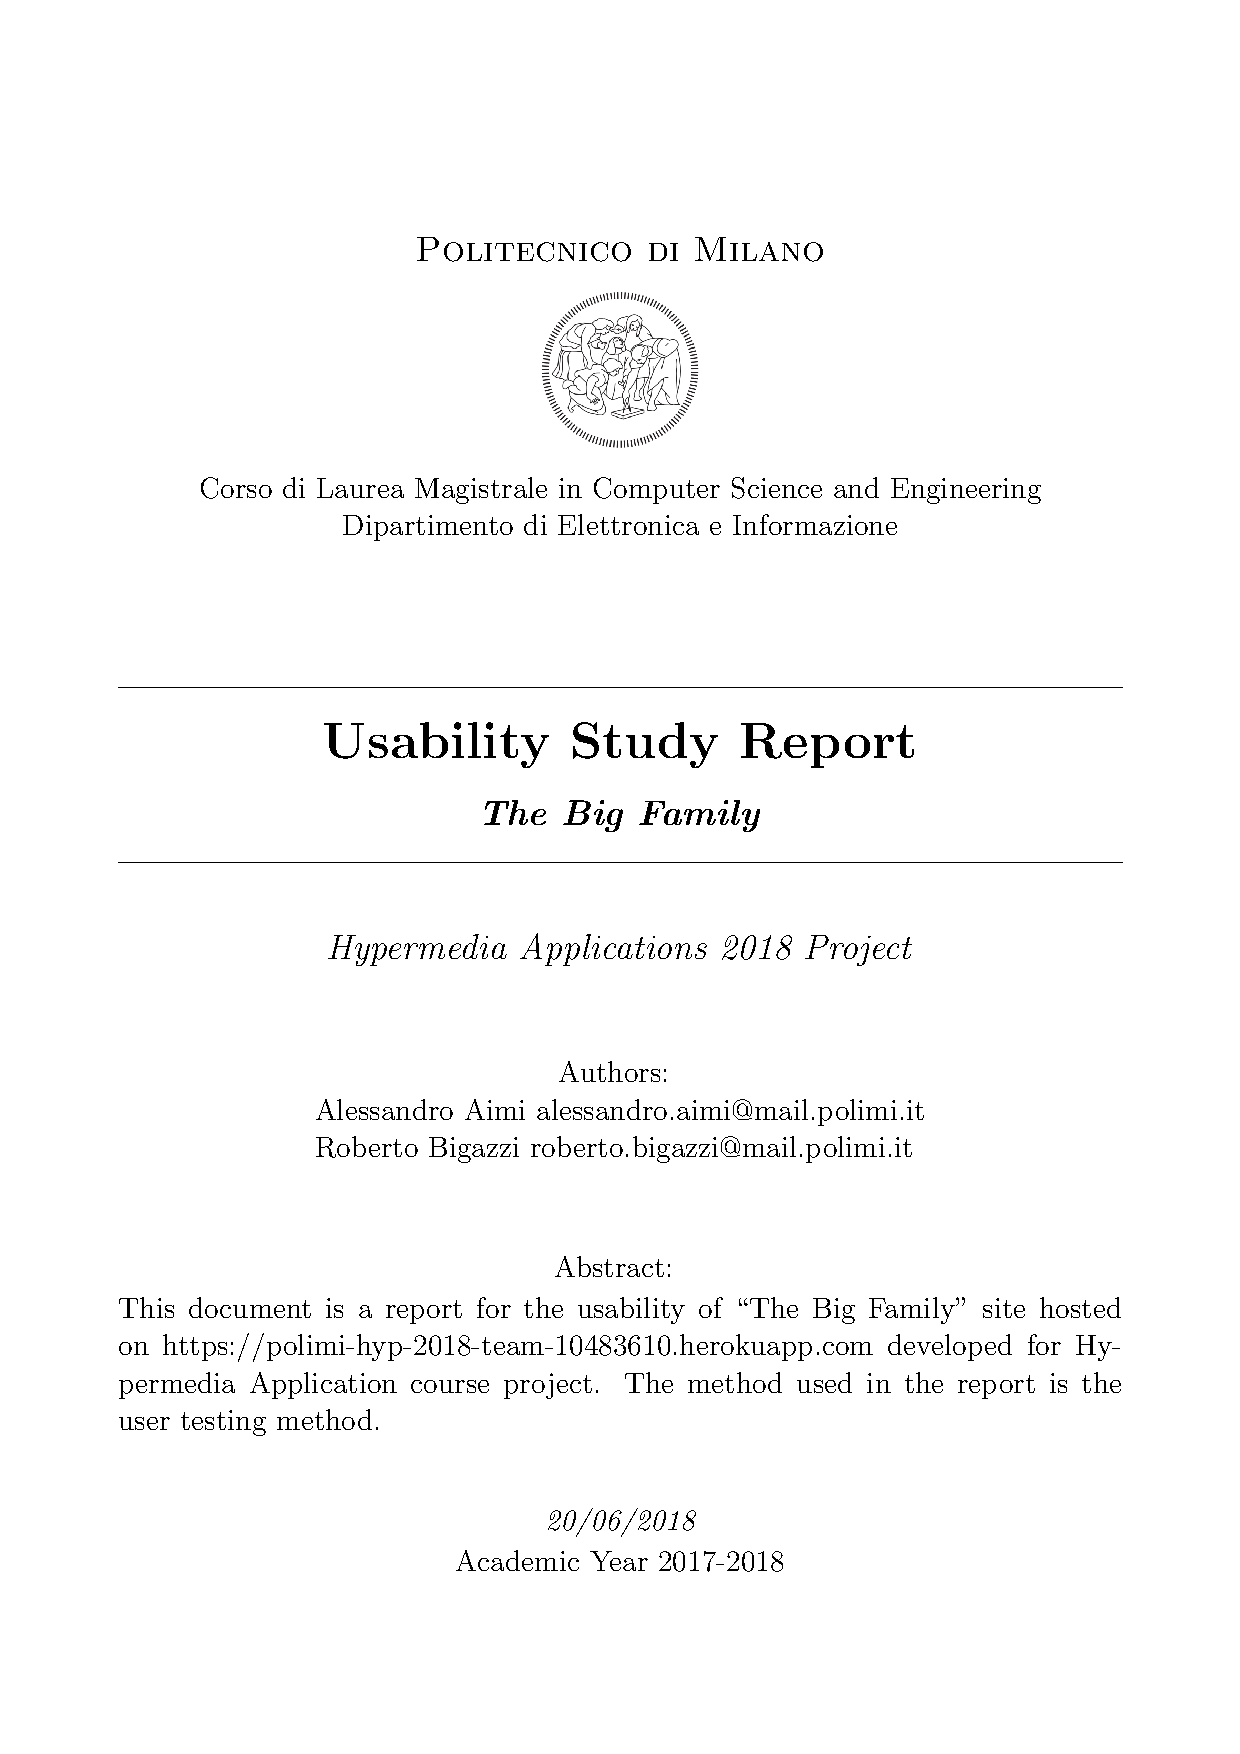
\includepdf[pages={1}]{FrontMatter/Frontispiece.pdf}
%
\let\cleardoublepage\clearpage
%
\clearpage
\setcounter{page}{1}
\pagenumbering{Roman}
\tableofcontents
%
%\input{FrontMatter/Colophon}
%
%\input{FrontMatter/Thanks}
%
%\input{FrontMatter/Dedication}
%
%\input{FrontMatter/Indexes}
%
%\input{FrontMatter/SommarioAbstract}
%
% ------------------------------------------------------------------------ %
% 	MAINMATTER
% ------------------------------------------------------------------------ %
%
\mainmatter
%
% ------------------------------------------------------------------------ %
% !TEX encoding = UTF-8
% !TEX TS-program = pdflatex
% !TEX root = ../Project.tex
% !TEX spellcheck = en-EN
% ------------------------------------------------------------------------ %
%
% ------------------------------------------------------------------------ %
% 	CHAPTER TITLE
% ------------------------------------------------------------------------ %
%
%
\chapter{Abstract}
%
%
% ------------------------------------------------------------------------ %
%
In this document will be presented, using various charts, the design on many levels of the website of an association for children with disabilities called ``The Big Family''. The purpose of the website is to introduce the association, its values and its services to the new users and to gather useful informations and contacts for people who already know it.
\linebreak
\linebreak
At first the website's content structure wil be presented using the Interactive Dialogue Model on three levels of abstraction. Than some fictional scenarios will be used to show some of the website features. Next the design-in-the-small of the site's pages is going to be explained through a low-fidelty wireframe fro each one of them, showing the basic visual organization of contents, navigation and interaction elements on the “screen”. In the end the database structure will be explained by the means of the Entity Relationship Model on two levels of abstraction.\\
\linebreak
The used software is:
\begin{itemize}

\item https://www.draw.io/ for the IDM and database schemas
\item https://wireframe.cc/ for the wireframes

\end{itemize}
%
% -----------------------------END------------------------------------- %

%
% ------------------------------------------------------------------------ %
% !TEX encoding = UTF-8
% !TEX TS-program = pdflatex
% !TEX root = ../Project.tex
% !TEX spellcheck = en-EN
% ------------------------------------------------------------------------ %
%
% ------------------------------------------------------------------------ %
% 	CHAPTER TITLE
% ------------------------------------------------------------------------ %
%
\chapter{Results}
%
% ------------------------------------------------------------------------ %
%
% -----------------------------END------------------------------------- %
%
% ------------------------------------------------------------------------ %
% !TEX encoding = UTF-8
% !TEX TS-program = pdflatex
% !TEX root = ../Project.tex
% !TEX spellcheck = en-EN
% ------------------------------------------------------------------------ %
%
% ------------------------------------------------------------------------ %
% 	CHAPTER TITLE
% ------------------------------------------------------------------------ %
%
\chapter{Discussion of results}
In the end we can say that it could be useful to change the page title ``Who We Are'' in something more like ``What Is The Association'' or ``History And Values'' to highlight the fact that the page is telling about the association, his history and his scope. Also we coul find a better position for the ``Contact Us'' landmark.
%
% -----------------------------END------------------------------------- %

%
%\appendix
%
%\input{MainMatter/Appendix}
%
% ------------------------------------------------------------------------ %
% 	BACKMATTER
% ------------------------------------------------------------------------ %
%
%\backmatter
%
%\input{BackMatter/Bibliography}
%
% ------------------------------------------------------------------------ %
% 	END DOCUMENT
% ------------------------------------------------------------------------ %
%
\end{document}
%
% ------------------------------------------------------------------------ %